% Options for packages loaded elsewhere
\PassOptionsToPackage{unicode}{hyperref}
\PassOptionsToPackage{hyphens}{url}
%
\documentclass[
]{article}
\usepackage{amsmath,amssymb}
\usepackage{lmodern}
\usepackage{iftex}
\ifPDFTeX
  \usepackage[T1]{fontenc}
  \usepackage[utf8]{inputenc}
  \usepackage{textcomp} % provide euro and other symbols
\else % if luatex or xetex
  \usepackage{unicode-math}
  \defaultfontfeatures{Scale=MatchLowercase}
  \defaultfontfeatures[\rmfamily]{Ligatures=TeX,Scale=1}
\fi
% Use upquote if available, for straight quotes in verbatim environments
\IfFileExists{upquote.sty}{\usepackage{upquote}}{}
\IfFileExists{microtype.sty}{% use microtype if available
  \usepackage[]{microtype}
  \UseMicrotypeSet[protrusion]{basicmath} % disable protrusion for tt fonts
}{}
\makeatletter
\@ifundefined{KOMAClassName}{% if non-KOMA class
  \IfFileExists{parskip.sty}{%
    \usepackage{parskip}
  }{% else
    \setlength{\parindent}{0pt}
    \setlength{\parskip}{6pt plus 2pt minus 1pt}}
}{% if KOMA class
  \KOMAoptions{parskip=half}}
\makeatother
\usepackage{xcolor}
\IfFileExists{xurl.sty}{\usepackage{xurl}}{} % add URL line breaks if available
\IfFileExists{bookmark.sty}{\usepackage{bookmark}}{\usepackage{hyperref}}
\hypersetup{
  pdftitle={100\_clasificacionFRE.R},
  pdfauthor={Daniel},
  hidelinks,
  pdfcreator={LaTeX via pandoc}}
\urlstyle{same} % disable monospaced font for URLs
\usepackage[margin=1in]{geometry}
\usepackage{color}
\usepackage{fancyvrb}
\newcommand{\VerbBar}{|}
\newcommand{\VERB}{\Verb[commandchars=\\\{\}]}
\DefineVerbatimEnvironment{Highlighting}{Verbatim}{commandchars=\\\{\}}
% Add ',fontsize=\small' for more characters per line
\usepackage{framed}
\definecolor{shadecolor}{RGB}{248,248,248}
\newenvironment{Shaded}{\begin{snugshade}}{\end{snugshade}}
\newcommand{\AlertTok}[1]{\textcolor[rgb]{0.94,0.16,0.16}{#1}}
\newcommand{\AnnotationTok}[1]{\textcolor[rgb]{0.56,0.35,0.01}{\textbf{\textit{#1}}}}
\newcommand{\AttributeTok}[1]{\textcolor[rgb]{0.77,0.63,0.00}{#1}}
\newcommand{\BaseNTok}[1]{\textcolor[rgb]{0.00,0.00,0.81}{#1}}
\newcommand{\BuiltInTok}[1]{#1}
\newcommand{\CharTok}[1]{\textcolor[rgb]{0.31,0.60,0.02}{#1}}
\newcommand{\CommentTok}[1]{\textcolor[rgb]{0.56,0.35,0.01}{\textit{#1}}}
\newcommand{\CommentVarTok}[1]{\textcolor[rgb]{0.56,0.35,0.01}{\textbf{\textit{#1}}}}
\newcommand{\ConstantTok}[1]{\textcolor[rgb]{0.00,0.00,0.00}{#1}}
\newcommand{\ControlFlowTok}[1]{\textcolor[rgb]{0.13,0.29,0.53}{\textbf{#1}}}
\newcommand{\DataTypeTok}[1]{\textcolor[rgb]{0.13,0.29,0.53}{#1}}
\newcommand{\DecValTok}[1]{\textcolor[rgb]{0.00,0.00,0.81}{#1}}
\newcommand{\DocumentationTok}[1]{\textcolor[rgb]{0.56,0.35,0.01}{\textbf{\textit{#1}}}}
\newcommand{\ErrorTok}[1]{\textcolor[rgb]{0.64,0.00,0.00}{\textbf{#1}}}
\newcommand{\ExtensionTok}[1]{#1}
\newcommand{\FloatTok}[1]{\textcolor[rgb]{0.00,0.00,0.81}{#1}}
\newcommand{\FunctionTok}[1]{\textcolor[rgb]{0.00,0.00,0.00}{#1}}
\newcommand{\ImportTok}[1]{#1}
\newcommand{\InformationTok}[1]{\textcolor[rgb]{0.56,0.35,0.01}{\textbf{\textit{#1}}}}
\newcommand{\KeywordTok}[1]{\textcolor[rgb]{0.13,0.29,0.53}{\textbf{#1}}}
\newcommand{\NormalTok}[1]{#1}
\newcommand{\OperatorTok}[1]{\textcolor[rgb]{0.81,0.36,0.00}{\textbf{#1}}}
\newcommand{\OtherTok}[1]{\textcolor[rgb]{0.56,0.35,0.01}{#1}}
\newcommand{\PreprocessorTok}[1]{\textcolor[rgb]{0.56,0.35,0.01}{\textit{#1}}}
\newcommand{\RegionMarkerTok}[1]{#1}
\newcommand{\SpecialCharTok}[1]{\textcolor[rgb]{0.00,0.00,0.00}{#1}}
\newcommand{\SpecialStringTok}[1]{\textcolor[rgb]{0.31,0.60,0.02}{#1}}
\newcommand{\StringTok}[1]{\textcolor[rgb]{0.31,0.60,0.02}{#1}}
\newcommand{\VariableTok}[1]{\textcolor[rgb]{0.00,0.00,0.00}{#1}}
\newcommand{\VerbatimStringTok}[1]{\textcolor[rgb]{0.31,0.60,0.02}{#1}}
\newcommand{\WarningTok}[1]{\textcolor[rgb]{0.56,0.35,0.01}{\textbf{\textit{#1}}}}
\usepackage{longtable,booktabs,array}
\usepackage{calc} % for calculating minipage widths
% Correct order of tables after \paragraph or \subparagraph
\usepackage{etoolbox}
\makeatletter
\patchcmd\longtable{\par}{\if@noskipsec\mbox{}\fi\par}{}{}
\makeatother
% Allow footnotes in longtable head/foot
\IfFileExists{footnotehyper.sty}{\usepackage{footnotehyper}}{\usepackage{footnote}}
\makesavenoteenv{longtable}
\usepackage{graphicx}
\makeatletter
\def\maxwidth{\ifdim\Gin@nat@width>\linewidth\linewidth\else\Gin@nat@width\fi}
\def\maxheight{\ifdim\Gin@nat@height>\textheight\textheight\else\Gin@nat@height\fi}
\makeatother
% Scale images if necessary, so that they will not overflow the page
% margins by default, and it is still possible to overwrite the defaults
% using explicit options in \includegraphics[width, height, ...]{}
\setkeys{Gin}{width=\maxwidth,height=\maxheight,keepaspectratio}
% Set default figure placement to htbp
\makeatletter
\def\fps@figure{htbp}
\makeatother
\setlength{\emergencystretch}{3em} % prevent overfull lines
\providecommand{\tightlist}{%
  \setlength{\itemsep}{0pt}\setlength{\parskip}{0pt}}
\setcounter{secnumdepth}{-\maxdimen} % remove section numbering
\ifLuaTeX
  \usepackage{selnolig}  % disable illegal ligatures
\fi

\title{100\_clasificacionFRE.R}
\author{Daniel}
\date{2021-10-08}

\begin{document}
\maketitle

\begin{Shaded}
\begin{Highlighting}[]
\FunctionTok{require}\NormalTok{(tidyverse)}
\end{Highlighting}
\end{Shaded}

\begin{verbatim}
## Loading required package: tidyverse
\end{verbatim}

\begin{verbatim}
## -- Attaching packages --------------------------------------- tidyverse 1.3.1 --
\end{verbatim}

\begin{verbatim}
## v ggplot2 3.3.5     v purrr   0.3.4
## v tibble  3.1.3     v dplyr   1.0.7
## v tidyr   1.1.3     v stringr 1.4.0
## v readr   2.0.0     v forcats 0.5.1
\end{verbatim}

\begin{verbatim}
## Warning: package 'dplyr' was built under R version 4.1.1
\end{verbatim}

\begin{verbatim}
## -- Conflicts ------------------------------------------ tidyverse_conflicts() --
## x dplyr::filter() masks stats::filter()
## x dplyr::lag()    masks stats::lag()
\end{verbatim}

\begin{Shaded}
\begin{Highlighting}[]
\FunctionTok{require}\NormalTok{(readxl)}
\end{Highlighting}
\end{Shaded}

\begin{verbatim}
## Loading required package: readxl
\end{verbatim}

\begin{Shaded}
\begin{Highlighting}[]
\FunctionTok{require}\NormalTok{(skimr)}
\end{Highlighting}
\end{Shaded}

\begin{verbatim}
## Loading required package: skimr
\end{verbatim}

\begin{verbatim}
## Warning: package 'skimr' was built under R version 4.1.1
\end{verbatim}

\begin{Shaded}
\begin{Highlighting}[]
\FunctionTok{require}\NormalTok{(PerformanceAnalytics)}
\end{Highlighting}
\end{Shaded}

\begin{verbatim}
## Loading required package: PerformanceAnalytics
\end{verbatim}

\begin{verbatim}
## Warning: package 'PerformanceAnalytics' was built under R version 4.1.1
\end{verbatim}

\begin{verbatim}
## Loading required package: xts
\end{verbatim}

\begin{verbatim}
## Loading required package: zoo
\end{verbatim}

\begin{verbatim}
## 
## Attaching package: 'zoo'
\end{verbatim}

\begin{verbatim}
## The following objects are masked from 'package:base':
## 
##     as.Date, as.Date.numeric
\end{verbatim}

\begin{verbatim}
## 
## Attaching package: 'xts'
\end{verbatim}

\begin{verbatim}
## The following objects are masked from 'package:dplyr':
## 
##     first, last
\end{verbatim}

\begin{verbatim}
## 
## Attaching package: 'PerformanceAnalytics'
\end{verbatim}

\begin{verbatim}
## The following object is masked from 'package:graphics':
## 
##     legend
\end{verbatim}

\begin{Shaded}
\begin{Highlighting}[]
\FunctionTok{require}\NormalTok{(factoextra)}
\end{Highlighting}
\end{Shaded}

\begin{verbatim}
## Loading required package: factoextra
\end{verbatim}

\begin{verbatim}
## Warning: package 'factoextra' was built under R version 4.1.1
\end{verbatim}

\begin{verbatim}
## Welcome! Want to learn more? See two factoextra-related books at https://goo.gl/ve3WBa
\end{verbatim}

\begin{Shaded}
\begin{Highlighting}[]
\NormalTok{data }\OtherTok{\textless{}{-}}
  \FunctionTok{read\_excel}\NormalTok{(}\FunctionTok{file.path}\NormalTok{(}
    \StringTok{\textquotesingle{}data\textquotesingle{}}\NormalTok{,}
    \StringTok{\textquotesingle{}raw\textquotesingle{}}\NormalTok{,}
    \StringTok{\textquotesingle{}ClasificacionFRE\textquotesingle{}}\NormalTok{,}
    \StringTok{\textquotesingle{}variablesClasificacionFRE.xlsx\textquotesingle{}}
\NormalTok{  ), }\AttributeTok{na =} \StringTok{\textquotesingle{}{-}\textquotesingle{}}\NormalTok{)}
\end{Highlighting}
\end{Shaded}

\begin{verbatim}
## New names:
## * Departamento -> Departamento...1
## * Departamento -> Departamento...2
\end{verbatim}

\begin{Shaded}
\begin{Highlighting}[]
\NormalTok{data }\SpecialCharTok{\%\textgreater{}\%}
  \FunctionTok{select}\NormalTok{(}\SpecialCharTok{!}\FunctionTok{contains}\NormalTok{(}\StringTok{\textquotesingle{}Departamento\textquotesingle{}}\NormalTok{)) }\SpecialCharTok{\%\textgreater{}\%} 
  \FunctionTok{chart.Correlation}\NormalTok{(., }\AttributeTok{histogram =} \ConstantTok{TRUE}\NormalTok{, }\AttributeTok{pch =} \DecValTok{19}\NormalTok{)}
\end{Highlighting}
\end{Shaded}

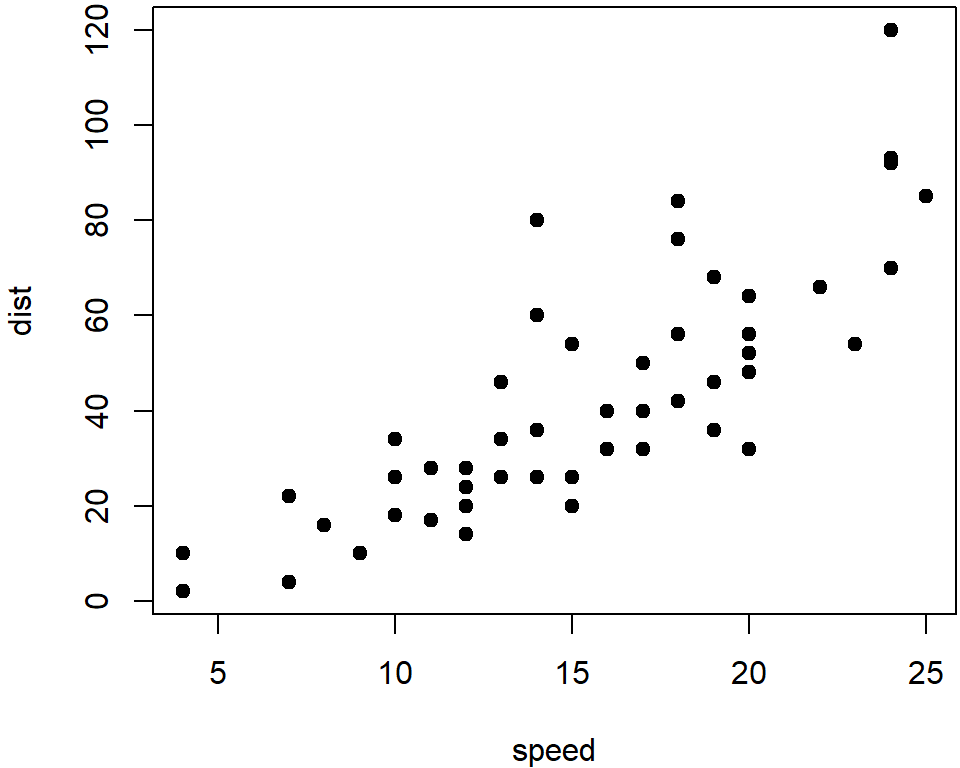
\includegraphics{100_clasificacionFRE_files/figure-latex/unnamed-chunk-1-1.pdf}

\begin{Shaded}
\begin{Highlighting}[]
\NormalTok{skimr}\SpecialCharTok{::}\FunctionTok{skim}\NormalTok{(data)}
\end{Highlighting}
\end{Shaded}

\begin{longtable}[]{@{}ll@{}}
\caption{Data summary}\tabularnewline
\toprule
\endhead
Name & data \\
Number of rows & 33 \\
Number of columns & 9 \\
\_\_\_\_\_\_\_\_\_\_\_\_\_\_\_\_\_\_\_\_\_\_\_ & \\
Column type frequency: & \\
character & 1 \\
numeric & 8 \\
\_\_\_\_\_\_\_\_\_\_\_\_\_\_\_\_\_\_\_\_\_\_\_\_ & \\
Group variables & None \\
\bottomrule
\end{longtable}

\textbf{Variable type: character}

\begin{longtable}[]{@{}lrrrrrrr@{}}
\toprule
skim\_variable & n\_missing & complete\_rate & min & max & empty &
n\_unique & whitespace \\
\midrule
\endhead
Departamento\ldots2 & 0 & 1 & 4 & 40 & 0 & 33 & 0 \\
\bottomrule
\end{longtable}

\textbf{Variable type: numeric}

\begin{longtable}[]{@{}
  >{\raggedright\arraybackslash}p{(\columnwidth - 20\tabcolsep) * \real{0.16}}
  >{\raggedleft\arraybackslash}p{(\columnwidth - 20\tabcolsep) * \real{0.05}}
  >{\raggedleft\arraybackslash}p{(\columnwidth - 20\tabcolsep) * \real{0.08}}
  >{\raggedleft\arraybackslash}p{(\columnwidth - 20\tabcolsep) * \real{0.07}}
  >{\raggedleft\arraybackslash}p{(\columnwidth - 20\tabcolsep) * \real{0.07}}
  >{\raggedleft\arraybackslash}p{(\columnwidth - 20\tabcolsep) * \real{0.07}}
  >{\raggedleft\arraybackslash}p{(\columnwidth - 20\tabcolsep) * \real{0.07}}
  >{\raggedleft\arraybackslash}p{(\columnwidth - 20\tabcolsep) * \real{0.07}}
  >{\raggedleft\arraybackslash}p{(\columnwidth - 20\tabcolsep) * \real{0.07}}
  >{\raggedleft\arraybackslash}p{(\columnwidth - 20\tabcolsep) * \real{0.07}}
  >{\raggedright\arraybackslash}p{(\columnwidth - 20\tabcolsep) * \real{0.22}}@{}}
\toprule
\begin{minipage}[b]{\linewidth}\raggedright
skim\_variable
\end{minipage} & \begin{minipage}[b]{\linewidth}\raggedleft
n\_missing
\end{minipage} & \begin{minipage}[b]{\linewidth}\raggedleft
complete\_rate
\end{minipage} & \begin{minipage}[b]{\linewidth}\raggedleft
mean
\end{minipage} & \begin{minipage}[b]{\linewidth}\raggedleft
sd
\end{minipage} & \begin{minipage}[b]{\linewidth}\raggedleft
p0
\end{minipage} & \begin{minipage}[b]{\linewidth}\raggedleft
p25
\end{minipage} & \begin{minipage}[b]{\linewidth}\raggedleft
p50
\end{minipage} & \begin{minipage}[b]{\linewidth}\raggedleft
p75
\end{minipage} & \begin{minipage}[b]{\linewidth}\raggedleft
p100
\end{minipage} & \begin{minipage}[b]{\linewidth}\raggedright
hist
\end{minipage} \\
\midrule
\endhead
Departamento\ldots1 & 0 & 1.00 & 1.700000e+01 & 9.670000e+00 &
1.000000e+00 & 9.000000e+00 & 1.700000e+01 & 2.50000e+01 & 3.300000e+01
& ▇▇▇▇▇ \\
Presupuesto\_2020 & 0 & 1.00 & 9.214848e+11 & 8.500217e+11 &
1.020000e+11 & 3.770000e+11 & 8.160000e+11 & 1.23900e+12 & 4.383000e+12
& ▇▃▁▁▁ \\
Presupuesto\_Salud\_2020 & 2 & 0.94 & 1.037347e+11 & 1.779548e+11 &
1.021624e+09 & 3.279217e+10 & 5.491663e+10 & 9.64771e+10 & 9.783884e+11
& ▇▁▁▁▁ \\
N\_productosCD\_2021 & 0 & 1.00 & 3.721000e+01 & 6.164000e+01 &
0.000000e+00 & 0.000000e+00 & 5.000000e+00 & 3.30000e+01 & 2.080000e+02
& ▇▁▁▁▁ \\
Cumplimiento\_A1\_2020-2021-06 & 0 & 1.00 & 9.800000e-01 & 7.000000e-02
& 7.500000e-01 & 1.000000e+00 & 1.000000e+00 & 1.00000e+00 &
1.000000e+00 & ▁▁▁▁▇ \\
Cumplimiento\_A2\_2020-2021-06 & 2 & 0.94 & 5.200000e-01 & 3.900000e-01
& 0.000000e+00 & 1.100000e-01 & 6.100000e-01 & 8.60000e-01 &
1.000000e+00 & ▇▂▁▅▇ \\
PropPortafolio & 0 & 1.00 & 8.400000e-01 & 1.900000e-01 & 3.500000e-01 &
8.200000e-01 & 9.400000e-01 & 1.00000e+00 & 1.000000e+00 & ▁▁▁▁▇ \\
No\_Inscritos & 2 & 0.94 & 1.593200e+02 & 2.144000e+02 & 1.000000e+00 &
2.650000e+01 & 7.800000e+01 & 2.22000e+02 & 1.054000e+03 & ▇▂▁▁▁ \\
\bottomrule
\end{longtable}

\begin{Shaded}
\begin{Highlighting}[]
\NormalTok{pca1 }\OtherTok{\textless{}{-}}\NormalTok{ data }\SpecialCharTok{\%\textgreater{}\%}
  \FunctionTok{drop\_na}\NormalTok{() }\SpecialCharTok{\%\textgreater{}\%} 
  \FunctionTok{column\_to\_rownames}\NormalTok{(}\StringTok{\textquotesingle{}Departamento...2\textquotesingle{}}\NormalTok{) }\SpecialCharTok{\%\textgreater{}\%} 
  \FunctionTok{select}\NormalTok{(}\SpecialCharTok{!}\FunctionTok{contains}\NormalTok{(}\StringTok{\textquotesingle{}Departamento\textquotesingle{}}\NormalTok{)) }\SpecialCharTok{\%\textgreater{}\%} 
  \FunctionTok{prcomp}\NormalTok{(., }\AttributeTok{scale =} \ConstantTok{TRUE}\NormalTok{, }\AttributeTok{center =} \ConstantTok{TRUE}\NormalTok{)}



\NormalTok{pca1 }\SpecialCharTok{\%\textgreater{}\%} \FunctionTok{plot}\NormalTok{()}
\end{Highlighting}
\end{Shaded}

\includegraphics{100_clasificacionFRE_files/figure-latex/unnamed-chunk-1-2.pdf}

\begin{Shaded}
\begin{Highlighting}[]
\FunctionTok{fviz\_pca\_ind}\NormalTok{(pca1,}
             \AttributeTok{col.ind =} \StringTok{"cos2"}\NormalTok{, }\CommentTok{\# Color by the quality of representation}
             \AttributeTok{gradient.cols =} \FunctionTok{c}\NormalTok{(}\StringTok{"\#00AFBB"}\NormalTok{, }\StringTok{"\#E7B800"}\NormalTok{, }\StringTok{"\#FC4E07"}\NormalTok{),}
             \AttributeTok{repel =} \ConstantTok{TRUE}     \CommentTok{\# Avoid text overlapping}
\NormalTok{)}
\end{Highlighting}
\end{Shaded}

\begin{verbatim}
## Warning: ggrepel: 1 unlabeled data points (too many overlaps). Consider
## increasing max.overlaps
\end{verbatim}

\includegraphics{100_clasificacionFRE_files/figure-latex/unnamed-chunk-1-3.pdf}

\begin{Shaded}
\begin{Highlighting}[]
\FunctionTok{fviz\_pca\_var}\NormalTok{(pca1,}
             \AttributeTok{col.var =} \StringTok{"contrib"}\NormalTok{, }\CommentTok{\# Color by contributions to the PC}
             \AttributeTok{gradient.cols =} \FunctionTok{c}\NormalTok{(}\StringTok{"\#00AFBB"}\NormalTok{, }\StringTok{"\#E7B800"}\NormalTok{, }\StringTok{"\#FC4E07"}\NormalTok{),}
             \AttributeTok{repel =} \ConstantTok{TRUE}     \CommentTok{\# Avoid text overlapping}
\NormalTok{)}
\end{Highlighting}
\end{Shaded}

\includegraphics{100_clasificacionFRE_files/figure-latex/unnamed-chunk-1-4.pdf}

\begin{Shaded}
\begin{Highlighting}[]
\NormalTok{clean\_data }\OtherTok{\textless{}{-}}\NormalTok{ data }\SpecialCharTok{\%\textgreater{}\%}
  \FunctionTok{drop\_na}\NormalTok{() }\SpecialCharTok{\%\textgreater{}\%} 
  \FunctionTok{column\_to\_rownames}\NormalTok{(}\StringTok{\textquotesingle{}Departamento...2\textquotesingle{}}\NormalTok{) }\SpecialCharTok{\%\textgreater{}\%} 
  \FunctionTok{select}\NormalTok{(}\SpecialCharTok{!}\FunctionTok{contains}\NormalTok{(}\StringTok{\textquotesingle{}Departamento\textquotesingle{}}\NormalTok{))}

\CommentTok{\# kmeans1 \textless{}{-} }
\NormalTok{funClusters }\OtherTok{\textless{}{-}} \ControlFlowTok{function}\NormalTok{(data, k) \{}
\NormalTok{  data }\SpecialCharTok{\%\textgreater{}\%}
    \FunctionTok{kmeans}\NormalTok{(k)}
\NormalTok{\}}
  

\NormalTok{k.values }\OtherTok{\textless{}{-}} \FunctionTok{data.frame}\NormalTok{(}\AttributeTok{k =} \DecValTok{1}\SpecialCharTok{:}\DecValTok{30}\NormalTok{)}

\NormalTok{k.values[}\StringTok{\textquotesingle{}TWITH\textquotesingle{}}\NormalTok{] }\OtherTok{\textless{}{-}} \FunctionTok{map\_dbl}\NormalTok{(k.values}\SpecialCharTok{$}\NormalTok{k, }\SpecialCharTok{\textasciitilde{}}\FunctionTok{funClusters}\NormalTok{(clean\_data, .x)}\SpecialCharTok{$}\NormalTok{tot.withinss)}

\NormalTok{k.values }\SpecialCharTok{\%\textgreater{}\%} 
  \FunctionTok{ggplot}\NormalTok{(}\FunctionTok{aes}\NormalTok{(}\AttributeTok{x =}\NormalTok{ k, }\AttributeTok{y =}\NormalTok{ TWITH)) }\SpecialCharTok{+} 
  \FunctionTok{geom\_point}\NormalTok{() }\SpecialCharTok{+} 
  \FunctionTok{geom\_line}\NormalTok{()}
\end{Highlighting}
\end{Shaded}

\includegraphics{100_clasificacionFRE_files/figure-latex/unnamed-chunk-1-5.pdf}

\begin{Shaded}
\begin{Highlighting}[]
\NormalTok{funClusters\_2 }\OtherTok{\textless{}{-}} \ControlFlowTok{function}\NormalTok{(data, k) \{}
\NormalTok{  t1 }\OtherTok{\textless{}{-}}\NormalTok{ data }\SpecialCharTok{\%\textgreater{}\%} 
    \FunctionTok{dist}\NormalTok{(}\AttributeTok{method =} \StringTok{\textquotesingle{}euclidean\textquotesingle{}}\NormalTok{) }\SpecialCharTok{\%\textgreater{}\%} 
    \FunctionTok{hclust}\NormalTok{(}\AttributeTok{method =} \StringTok{\textquotesingle{}complete\textquotesingle{}}\NormalTok{)}
  
\NormalTok{  t2 }\OtherTok{\textless{}{-}} \FunctionTok{cutree}\NormalTok{(t1, k)}
  \FunctionTok{return}\NormalTok{(}\FunctionTok{list}\NormalTok{(}\AttributeTok{clust =}\NormalTok{ t1, }\AttributeTok{tree =}\NormalTok{ t2))}
\NormalTok{\}}



\FunctionTok{plot}\NormalTok{(}\FunctionTok{funClusters\_2}\NormalTok{(clean\_data, }\DecValTok{3}\NormalTok{)}\SpecialCharTok{$}\NormalTok{clust, }\AttributeTok{cex =} \FloatTok{0.6}\NormalTok{, }\AttributeTok{hang =} \SpecialCharTok{{-}}\DecValTok{1}\NormalTok{)}
\end{Highlighting}
\end{Shaded}

\includegraphics{100_clasificacionFRE_files/figure-latex/unnamed-chunk-1-6.pdf}

\begin{Shaded}
\begin{Highlighting}[]
\NormalTok{clean\_data }\SpecialCharTok{\%\textgreater{}\%} 
\NormalTok{  \{}\FunctionTok{fviz\_cluster}\NormalTok{(}\FunctionTok{list}\NormalTok{(}\AttributeTok{data =}\NormalTok{ ., }\AttributeTok{cluster =} \FunctionTok{funClusters\_2}\NormalTok{(., }\DecValTok{5}\NormalTok{)}\SpecialCharTok{$}\NormalTok{tree))\}}
\end{Highlighting}
\end{Shaded}

\includegraphics{100_clasificacionFRE_files/figure-latex/unnamed-chunk-1-7.pdf}

\begin{Shaded}
\begin{Highlighting}[]
\CommentTok{\# stats::cutree(:, k = 4) \%\textgreater{}\% }
  \CommentTok{\# as.data.frame() \%\textgreater{}\% }
  \CommentTok{\# dplyr::rename(.,cluster\_group = .) \%\textgreater{}\%}
  \CommentTok{\# tibble::rownames\_to\_column("type\_col")}
  \CommentTok{\# }
\end{Highlighting}
\end{Shaded}


\end{document}
